\documentclass[spanish,a4paper,14pt,oneside]{extreport}

%%%%%%%%%%%%%%%%%%%%%%%%%%%%%%%%%%%%%%%%%%%%%%%%%%%%%%%%%%%%%%%%%%%%%%%%%%%%%%%
\usepackage[dvips]{graphicx}
\usepackage[dvips]{epsfig}
\usepackage[utf8]{inputenc}
\usepackage{listings}
\usepackage[spanish]{babel}
\usepackage{eurosym}
\usepackage{alltt}
\usepackage{algorithm}
\usepackage{algorithmic}
\usepackage{multirow}
\usepackage[top=2cm, bottom=2cm, left=2cm, right=2cm]{geometry}
%%%%%%%%%%%%%%%%%%%%%%%%%%%%%%%%%%%%%%%%%%%%%%%%%%%%%%%%%%%%%%%%%%%%%%%%%%%%%%%

\newcommand{\SONY}{{\sc Sony}}
\newcommand{\MICROSOFT}{{\sc Microsoft}}
\newcommand{\GCC}{\textsf{\textsc{G}CC}}
\newcommand{\INTEL}{\textsf{\textsc{I}ntel}}

%%% Traducimos el pseudocodigo
\renewcommand{\algorithmicwhile}{\textbf{mientras}}
\renewcommand{\algorithmicend}{\textbf{fin}}
\renewcommand{\algorithmicdo}{\textbf{hacer}}
\renewcommand{\algorithmicif}{\textbf{si}}
\renewcommand{\algorithmicthen}{\textbf{entonces}}
\renewcommand{\algorithmicrepeat}{\textbf{repetir}}
\renewcommand{\algorithmicuntil}{\textbf{hasta que}}
\renewcommand{\algorithmicelse}{\textbf{en otro caso}}
\renewcommand{\algorithmicfor}{\textbf{para}}

%\newcommand{\RETURN}{\textbf{retornar} }
\newcommand{\RET}{\STATE \textbf{retornar} }
\newcommand{\TO}{\textbf{hasta} }
\newcommand{\AND}{\textbf{y} }
\newcommand{\OR}{\textbf{o} }

%%%%%%%%%%%%%%%%% Creamos un entorno para listar código fuente %%%%%%%%%%%%%%%
\newenvironment{sourcecode}
{\begin{list}{}{\setlength{\leftmargin}{1em}}\item\scriptsize\bfseries}
{\end{list}}

\newenvironment{littlesourcecode}
{\begin{list}{}{\setlength{\leftmargin}{1em}}\item\tiny\bfseries}
{\end{list}}

\newenvironment{summary}
{\par\noindent\begin{center}\textbf{Abstract}\end{center}\begin{itshape}\par\noindent}
{\end{itshape}}

\newenvironment{keywords}
{\begin{list}{}{\setlength{\leftmargin}{1em}}\item[\hskip\labelsep \bfseries Keywords:]}
{\end{list}}

\newenvironment{palabrasClave}
{\begin{list}{}{\setlength{\leftmargin}{1em}}\item[\hskip\labelsep \bfseries Palabras clave:]}
{\end{list}}


%%%%%%%%%%%%%%%%%%%%%%%%%%%%%%%%%%%%%%%%%%%%%%%%%%%%%%%%%%%%%%%%%%%%%%%%%%%%%%%
% Format
%%%%%%%%%%%%%%%%%%%%%%%%%%%%%%%%%%%%%%%%%%%%%%%%%%%%%%%%%%%%%%%%%%%%%%%%%%%%%%%
%\usepackage{showframe}
%\marginparwidth 0mm
%%\topmargin -4 mm
%\topmargin -21 mm
%\headheight 10 mm
%\headsep 10 mm

%\textheight 229 mm
%\textheight 246 mm

%\oddsidemargin -5.4 mm
%\evensidemargin -5.4 mm
%\oddsidemargin 5 mm
%\evensidemargin 5 mm

%\oddsidemargin -3 mm
%\evensidemargin -3 mm

%\textwidth 17 cm
%\textwidth 15 cm
%\columnsep 10 mm

\input{amssym.def}

%%%%%%%%%%%%%%%%%%%%%%%%%%%%%%%%%%%%%%%%%%%%%%%%%%%%%%%%%%%%%%%%%%%%%%%%%%%%%%%

\begin{document}

%%%%%%%%%%%%%%%%%%%%%%%%%%%%%%%%%%%%%%%%%%%%%%%%%%%%%%%%%%%%%%%%%%%%%%%%%%%%%%%
% First Page
%%%%%%%%%%%%%%%%%%%%%%%%%%%%%%%%%%%%%%%%%%%%%%%%%%%%%%%%%%%%%%%%%%%%%%%%%%%%%%%

\pagestyle{empty}
\thispagestyle{empty}


\newcommand{\HRule}{\rule{\linewidth}{1mm}}
\setlength{\parindent}{0mm}
\setlength{\parskip}{0mm}

\vspace*{\stretch{0.5}}

\begin{center}

\includegraphics[scale=0.8]{images/logo_vertical}\\[10mm]
{\Huge Trabajo de Fin de Grado}
\end{center}

\HRule
\begin{flushright}
        {\Huge Simulador didáctico de arquitectura de computadores} \\[2.5mm]
        {\Large \textit{Didactic simulator for Computer Architecture} .} \\[5mm]
        {\Large Adrián Abreu González} \\[5mm]


\end{flushright}
\HRule
\vspace*{\stretch{2}}
\begin{center}
  \Large La Laguna, \today
\end{center}

\setlength{\parindent}{5mm}

%%%%%%%%%%%%%%%%%%%%%%%%%%%%%%%%%%%%%%%%%%%%%%%%%%%%%%%%%%%%%%%%%%%%%%%%%%%%%%%
% Signature page (add the official stamp)
%%%%%%%%%%%%%%%%%%%%%%%%%%%%%%%%%%%%%%%%%%%%%%%%%%%%%%%%%%%%%%%%%%%%%%%%%%%%%%%
\newpage
%\cleardoublepage
\thispagestyle{empty}

D. {\bf Iván Castilla Rodríguez}, con N.I.F. 78.565.451-G
profesor
Titular de Universidad
adscrito al Departamento
de Nombre del Departamento
de la Universidad de La Laguna, como tutor

\bigskip
\bigskip
{\bf C E R T I F I C A}

\bigskip
\bigskip
\bigskip
Que la presente memoria titulada:

\bigskip
``{\it Simulador didáctico de arquitectura de computadores.}''

\bigskip
\bigskip
\bigskip

\noindent ha sido realizada bajo su dirección por D. {\bf Adrián Abreu González},
con N.I.F. 54.111.250-R.

\bigskip
\bigskip

Y para que así conste, en cumplimiento de la legislación vigente y a los efectos
oportunos firman la presente en La Laguna a \today

%\cleardoublepage
\newpage
%%%%%%%%%%%%%%%%%%%%%%%%%%%%%%%%%%%%%%%%%%%%%%%%%%%%%%%%%%%%%%%%%%%%%%%%%%%%%%%
\thispagestyle{empty}

{ \flushright

\begin{LARGE}
Agradecimientos
\end{LARGE}

\hspace{3mm}

\begin{large}


\hspace{3mm}
XXX

\hspace{3mm}
XXX


\hspace{3mm}
XXX


\hspace{3mm}
XXX


\end{large}

}

%%%%%%%%%%%%%%%%%%%%%%%%%%%%%%%%%%%%%%%%%%%%%%%%%%%%%%%%%%%%%%%%%%%%%%%%%%%%%%%%%
\newpage

\begin{huge}
Licencia
\end{huge}

\bigskip
\begin{center}

\includegraphics[scale=1.5]{images/by_88x31}\\[10mm]
{\Large \copyright~Esta obra está bajo una licencia de Creative Commons Reconocimiento 4.0 Internacional.
}
\end{center}



%%%%%%%%%%%%%%%%%%%%%%%%%%%%%%%%%%%%%%%%%%%%%%%%%%%%%%%%%%%%%%%%%%%%%%%%%%%%%%%
\newpage  %\cleardoublepage
\begin{abstract}
{\em

El objetivo de este trabajo ha sido ....
%
bla, bla, bla
%
bla, bla, bla
%
bla, bla, bla

\bigskip
La competencia [E6], que figura en la guía docente, indica que en la memoria del trabajo se ha de incluir:
antecedentes, problemática o estado del arte, objetivos, fases y desarrollo del proyecto,
conclusiones, y líneas futuras.


\bigskip
Se ha incluido el apartado de 'Licencia' con todas las posibles licencias abiertas (Creative Commons).
En el caso en que se decida hacer público el contenido de la memoria, habrá que elegir una de ellas
(y borrar las demás).
La decisión de hacer pública o no la memoria se indica en el momento de subir la memoria a la Sede Electrónica de la ULL, paso necesario en el proceso de presentación del TFG.

\bigskip
El documento de memoria debe tener un máximo de 50 páginas.

\bigskip
No se deben dejar páginas en blanco al comenzar un capítulo, ya que
el documento no está pensado para se impreso sino visionado
con un lector de PDFs.

\bigskip
También es recomendable márgenes pequeños ya que, al firmar digitalmente por
la Sede, se coloca un marco alrededor del texto original.


\bigskip
El tipo de letra base ha de ser de 14ptos.
}

\begin{palabrasClave}
Palabra reservada1, Palabra reservada2, ...
\end{palabrasClave}

\end{abstract}
%%%%%%%%%%%%%%%%%%%%%%%%%%%%%%%%%%%%%%%%%%%%%%%%%%%%%%%%%%%%%%%%%%%%%%%%%%%%%%%

%%%%%%%%%%%%%%%%%%%%%%%%%%%%%%%%%%%%%%%%%%%%%%%%%%%%%%%%%%%%%%%%%%%%%%%%%%%%%%%
\newpage  %\cleardoublepage
\begin{summary}
{\em

Here should be the abstract in a foreing language...

}

\begin{keywords}
Keyword1, Keyword2, Keyword3, ...
\end{keywords}

\end{summary}
%%%%%%%%%%%%%%%%%%%%%%%%%%%%%%%%%%%%%%%%%%%%%%%%%%%%%%%%%%%%%%%%%%%%%%%%%%%%%%%

%%%%%%%%%%%%%%%%%%%%%%%%%%%%%%%%%%%%%%%%%%%%%%%%%%%%%%%%%%%%%%%%%%%%%%%%%%%%%%%
\newpage{\pagestyle{empty}}
\thispagestyle{empty}

%%%%%%%%%%%%%%%%%%%%%%%%%%%%%%%%%%%%%%%%%%%%%%%%%%%%%%%%%%%%%%%%%%%%%%%%%%%%%%%


\pagestyle{myheadings} %my head defined by markboth or markright
% No funciona bien \markboth sin "twoside" en \documentclass, pero al
% ponerlo se dan un montón de errores de underfull \vbox, con lo que no se
% ha puesto.
\markboth{Adrián Abreu González}{Simulador didáctico de arquitectura de computadores}

%%%%%%%%%%%%%%%%%%%%%%%%%%%%%%%%%%%%%%%%%%%%%%%%%%%%%%%%%%%%%%%%%%%%%%%%%%%%%%%
%Numeracion en romanos
\renewcommand{\thepage}{\roman{page}}
\setcounter{page}{1}

%%%%%%%%%%%%%%%%%%%%%%%%%%%%%%%%%%%%%%%%%%%%%%%%%%%%%%%%%%%%%%%%%%%%%%%%%%%%%%%

\tableofcontents

%%%%%%%%%%%%%%%%%%%%%%%%%%%%%%%%%%%%%%%%%%%%%%%%%%%%%%%%%%%%%%%%%%%%%%%%%%%%%%%
\newpage{\pagestyle{empty}}

\listoffigures

%%%%%%%%%%%%%%%%%%%%%%%%%%%%%%%%%%%%%%%%%%%%%%%%%%%%%%%%%%%%%%%%%%%%%%%%%%%%%%%
\newpage{\pagestyle{empty}}

\listoftables

%%%%%%%%%%%%%%%%%%%%%%%%%%%%%%%%%%%%%%%%%%%%%%%%%%%%%%%%%%%%%%%%%%%%%%%%%%%%%%%
\newpage{\pagestyle{empty}}

%%%%%%%%%%%%%%%%%%%%%%%%%%%%%%%%%%%%%%%%%%%%%%%%%%%%%%%%%%%%%%%%%%%%%%%%%%%%%%%
%Numeracion a partir del capitulo I
\renewcommand{\thepage}{\arabic{page}}
\setcounter{page}{1}


\chapter{Introducción}
\label{chapter:intro}

%%%%%%%%%%%%%%%%%%%%%%%%%%%%%%%%%%%%%%%%%%%%%%%%%%%%%%%%%%%%%%%%%%%%%%%%%%%%%
% Chapter 1: Introducción 
%%%%%%%%%%%%%%%%%%%%%%%%%%%%%%%%%%%%%%%%%%%%%%%%%%%%%%%%%%%%%%%%%%%%%%%%%%%%%%%

%---------------------------------------------------------------------------------
\section{Introducción}
\label{1:sec:1}
El peso de la tecnología en la eficiencia de los computadores actuales es innegable. Sin embargo, los 
conceptos básicos que definen la arquitectura de estos computadores se basan en ideas de hace varias décadas.
Sin embargo, en el ámbito docente, resulta difícil transmitir estos fundamentos, ya que han quedado superpuestos
por el aumento de la complejidad de la arquitectura, haciendo que sea imprescindible una gran abstracción por 
parte del alumno al no poder disponer de las máquinas originales en los que se implementaron.

\bigskip
Las herramientas docentes típicas, como pueden ser una pizarra, un libro de texto
o diapositivas, tienen una capacidad limitada para representar los fundamentos
ya expuestos.

\bigskip
Este trabajo se centra en el uso de simuladores como medio de apoyo docente para el 
tema del  paralelismo a nivel de instrucción, una parte fundamental en el incremento
de rendimiento de las computadoras.

\bigskip
En este contexto, los simuladores juegan una pieza clave en el campo de la Arquitectura de Computadores,
permitiendo asociar fundamentos y teorías, simplificando abstracciones y facilitando la labor docente.


%---------------------------------------------------------------------------------
\section{Paralelismo a nivel de instrucción}
\label{1:sec:2}
Con el objetivo de mejorar el rendimiento de una computadora es necesario superar la barrera
de 1 ciclo por instrucción -el límite máximo que se puede conseguir con la técnica de segmentación-,
para ello, se debe conseguir ejecutar varias instrucciones diferentes de forma paralela.

\bigskip
Para alcanzar este propósito se deben considerar varios factores:

\begin{itemize}

\item Se debe proveer de una estructura capaz de emitir múltiples instrucciones.

\item Se deben detectar los posibles riesgos asociados (tanto entre las instrucciones que se van a 
emitir entre sí como entre las que se van a emitir y las que ya están ejecutándose). 

\item Se debe hacer una planificación para evitar que sucedan los posibles riesgos de datos o 
de estructuras, y también optimizar el funcionando de la máquina.

\end{itemize}

\bigskip
Existen dos grandes técnicas para conseguir explotar el paralelismo a nivel de instrucción:

\begin{enumerate}

\item \textbf{Planificación dinámica}: La responsabilidad de detectar y resolver los problemas recae
en el propio hardware.

\item \textbf{Planificación estática}: Delega las decisiones en el software. Manteniendo un hardware
relativamente simple.

\end{enumerate}

\subsection{Superescalar}

La mayoría de máquinas Superescalares hacen uso de la planificación dinámica, es decir, el hardware 
en sí mismo es el encargado de mantener la emisión de múltiples instrucciones, decodificarlas y 
ejecutarlas.

\bigskip
Para resolver los problemas de dependencias se utiliza una modificación del algoritmo de Tomasulo.
Este algoritmo nació originnalmente con el objetivo de controlar las dependencias en la unidad
funcional de punto flotante de la máquina 360/91 de IBM.

\bigskip
Mediante un seguimiento de los operandos y renombrado de registros se eliminaron los tres tipos 
de dependencias \textit{Read After Write}, \textit{Write After Read} y \textit{Write After Write}. 

\bigskip
Las máquinas superescalares incorporan nuevas estructuras de hardware como el ReorderBuffer para
permitir la ejecución fuera de orden.

\subsection{VLIW}

A diferencia de las máquinas Superescalares, las máquinas \textit{Very Long Instruction Word},
mantienen un hardware simple de emisión y todas las responsabilidades caen en el compilador.

\bigskip
Para mantener este hardware simple, estas máquinas trabajan como su propio nombre indica, con
un tamaño de palabra muy grande, es decir, las instrucciones de la máquina son un "grupo"
de instrucciones normales que pueden ejecutarse en paralelo.

\bigskip
Esto por supuesto, implica una serie de ventaja / inconvenientes. Por una parte, el compilador,
debe tener una visión completa del programa, conlleva un nivel de complejidad elevado y requiere
un alto grado de especialización por máquina para poder realizar las mayores optimizacions posibles.

\bigskip
Por otra parte, sin embargo, el software es versátil y la circuitería al ser de una menor complejidad 
permite mayores velocidades de reloj.

%---------------------------------------------------------------------------------
\section{Motivación para el trabajo}
\label{1:sec:3}
Como se ha mencionado, el uso de un simulador para apoyar la docencia de esta área
de Arquitectura de Computadores resultaba un campo realmente interesante y relevante. 
De hecho, un simulador que cumpla estas características, ya existe. El actual profesor 
de la Universidad de La Laguna Iván Castilla desarrolló un simulador en C++ con este propósito.

\bigskip
Este simulador se ha estado utilizando como un complemento fundamental en la docencia
de Arquitectura de Computadores, pero con el paso del tiempo, ha quedado obsoleto. 
No tanto por su funcionalidad, puesto que los fundamentos teóricos sobre los que 
se basa no han cambiado con el tiempo, como por su aspecto visual y su accesibilidad.

\bigskip
Es por esto se ha querido recuperar esta herramienta para continuar con su desarrollo 
y ampliación y este trabajo de fin de grado se centra en migrar esta aplicación a versión 
web de tal forma que sirva como base para los futuros proyectos.



%%%%%%%%%%%%%%%%%%%%%%%%%%%%%%%%%%%%%%%%%%%%%%%%%%%%%%%%%%%%%%%%%%%%%%%%%%%%%%%

\chapter{Antecedentes}
\label{chapter:dos}

%%%%%%%%%%%%%%%%%%%%%%%%%%%%%%%%%%%%%%%%%%%%%%%%%%%%%%%%%%%%%%%%%%%%%%%%%%%%%%%
% Chapter 2: Antecedentes
%%%%%%%%%%%%%%%%%%%%%%%%%%%%%%%%%%%%%%%%%%%%%%%%%%%%%%%%%%%%%%%%%%%%%%%%%%%%%%%

%++++++++++++++++++++++++++++++++++++++++++++++++++++++++++++++++++++++++++++++

\section{SIMDE}
\label{2:sec1}
En el año dos mil cuatro, el por aquel entonces estudiante de esta universidad, 
Iván Castilla Rodríguez - y ahora tutor de este trabajo de fin de grado-, 
desarrolló como proyecto final de carrera un Simulador didáctico para la enseñanza 
de arquitectura de computadores, el cual fue bautizado como Simde. \cite{SIMDE}

\bigskip
Este simulador como se ha comentado en el apartado 1.4 cumple con las características
deseadas y esperadas de un simulador para la docencia de este ámbito.

\bigskip
Sin embargo, esta herramienta ya se encuentra desfasada. No ha sido un proyecto en constante
evolución, fue diseñada utilizando C++98 y C++ Builder y el código ahora mismo no resultaría
fácil de adaptar y mantener.

\begin{figure}[!th]
\begin{center}
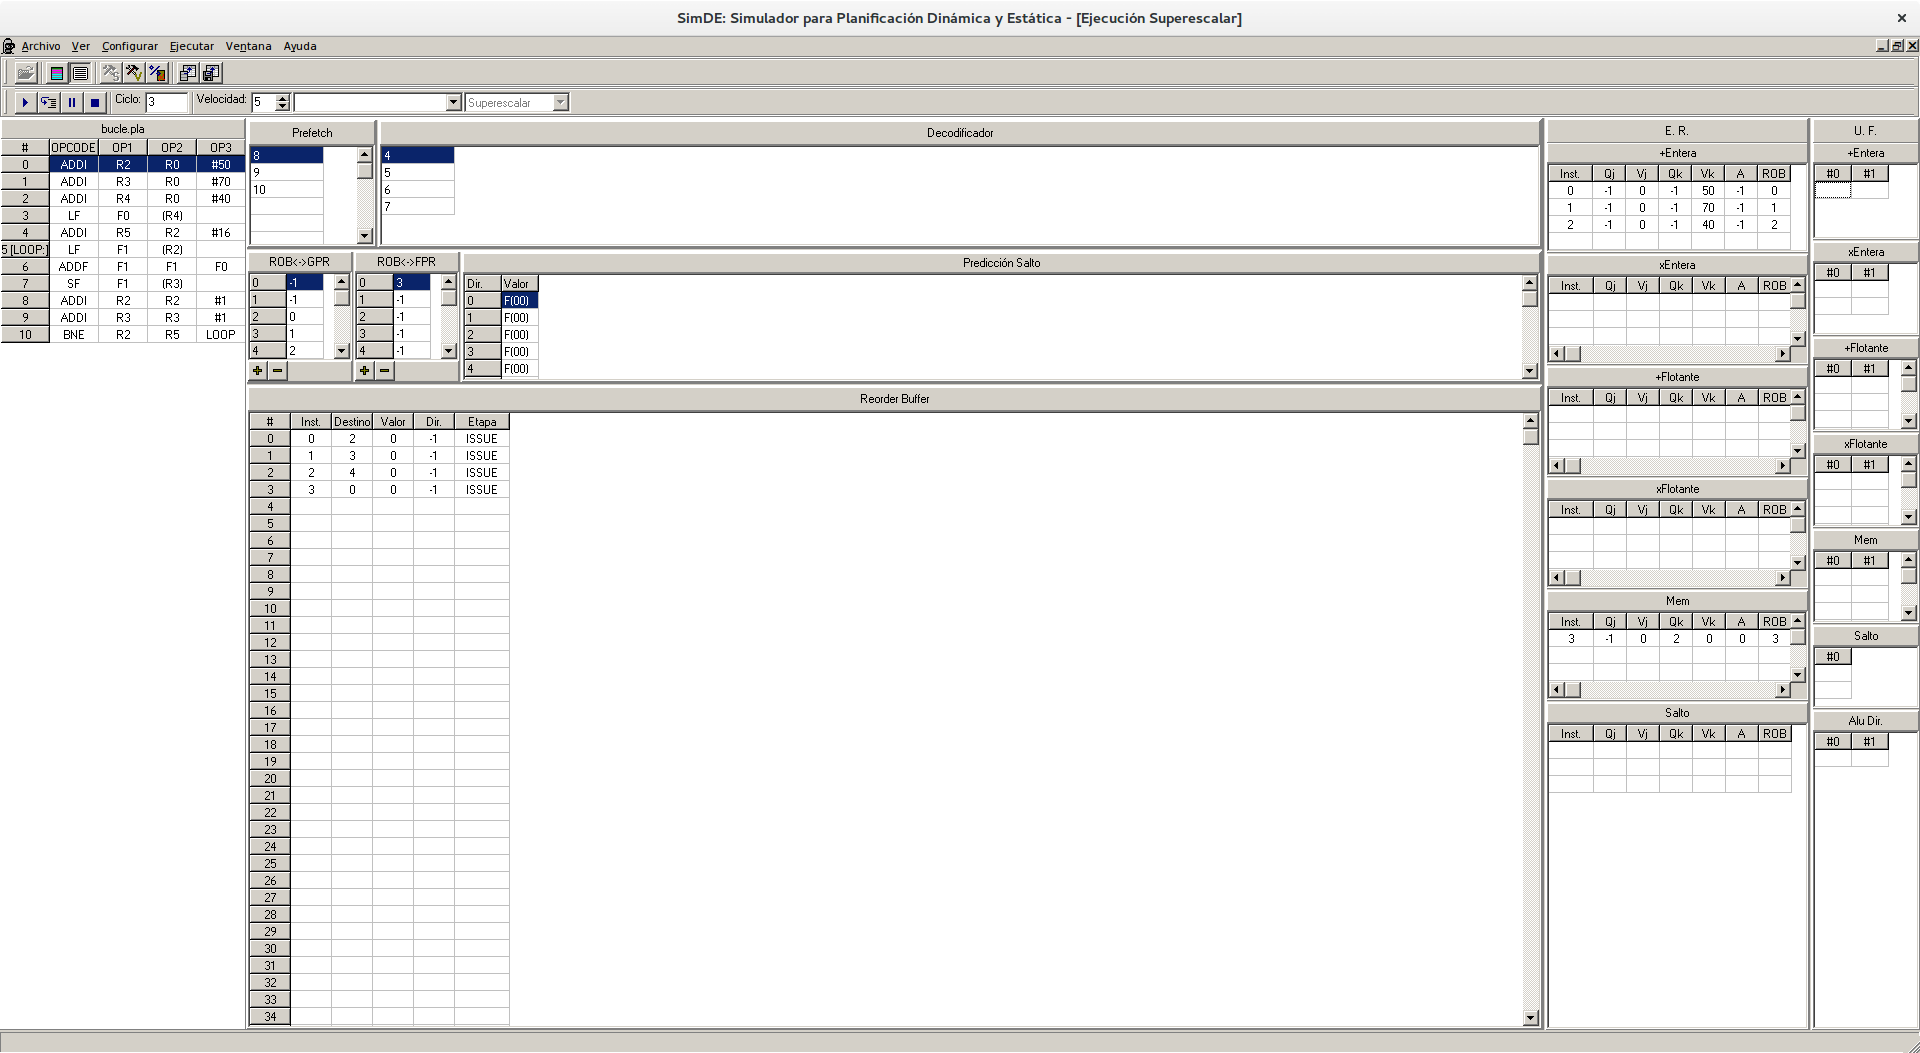
\includegraphics[width=0.8\textwidth]{images/cap2/simdeoriginal.eps}
\caption{Simulador original SIMDE}
\label{fig:Simulador original SIMDE}
\end{center}
\end{figure}

\section{Otros simuladores}
\label{2:sec2}
Sería irrazonable embarcarse en la tarea de migrar SIMDE sin comprobar antes si ya existe alguna
herramienta que se adapte a estas necesidades.

\begin{center}
    \begin{tabular}{| l | p{12cm} |}
    \hline
    Simulador & Descripción \\ \hline
    SESC & Simulador de máquinas Superescalares desarrollado en la Universidad de Illinois, posee
    características tan interesantes como el SMT, el CMP... Pero carece de interfaz gráfica. \\ \hline
    ReSIM & Este simulador de máquinas Superescalares está basado en la ejecución por trazas. Se encuentra 
    disponible para múltiples dispositivos Xilink. \\ \hline
    VLIW-DLX & Basado en WinDLX y desarrollado en la Universidad de praga, intenta aportar un conocimiento 
    detallado de las máquinas VLIW. \\ \hline
    \end{tabular}
\end{center}

Como vemos, aunque existen múltiples simuladores dentro de esta sección, ninguno cumple con el objetivo inicial,
es más, lamentablemente, la mayoría de los simuladores tienen más de una década y NINGUNO de los mencionados se 
encuentra disponible en versión web.

\section{Evolución del mundo web}
\label{2:sec3}
A modo de curiosidad, en el proyecto original, se consideraba poco factible la realización de 
un simulador de estas características en el entorno debido al escaso rendimiento. Cito textualmente:

\begin{quotation}
Utilizar programación web. Pese a las muchas ventajas de la programación
web en aspectos como la distribución y accesibilidad del programa, la realidad
es que el uso que se iba a dar a esta herramienta no invitaba a la utilización de
esta opción. El simulador no estaba planteado como una herramienta con
arquitectura cliente-servidor, ni tampoco se pretendía una ejecución distribuida.
La idea era que se procesara en la máquina del alumno y no en un servidor. El
uso de applets de java tampoco era una opción atractiva debido a la lentitud de
ejecución de java por ser interpretado.
\end{quotation} \cite{SIMDE}

\bigskip
Por sorprendete que resulte, este argumento totalmente justificado y válido en el momento
de su enunciado, resulta difícil de defender en un contexto actual. Hoy en día,
el rendimiento del lenguaje Javascript en el navegador es increíblemente alto. Y si vemos que la diferencia 
de este texto a ahora, es de unos escasos trece años -aunque ciertamenta nada despreciables en el mundo 
tecnológico, la diferencia resulta asombrosa.
 
\bigskip
Si intentamos encontrar un origen para esta diferencia tan increíble de rendimiento, sin duda
debemos remontar a la aparición de las primeras grandes aplicaciones que hacen uso de la tecnología
\textit{Ajax} como por ejemplo Gmail. La tendencia a diseñar más y más aplicaciones utilizando esta
tecnología resultó en una guerra por aumentar el rendimiento por parte de los distintos navegadores. \cite{EvolutionJavascript}





%%%%%%%%%%%%%%%%%%%%%%%%%%%%%%%%%%%%%%%%%%%%%%%%%%%%%%%%%%%%%%%%%%%%%%%%%%%%%%%
\newpage{\pagestyle{empty}}
\thispagestyle{empty}

\chapter{Tecnologías}
\label{chapter:tres}

%%%%%%%%%%%%%%%%%%%%%%%%%%%%%%%%%%%%%%%%%%%%%%%%%%%%%%%%%%%%%%%%%%%%%%%%%%%%%%%
% Chapter 3: Tecnologías
%%%%%%%%%%%%%%%%%%%%%%%%%%%%%%%%%%%%%%%%%%%%%%%%%%%%%%%%%%%%%%%%%%%%%%%%%%%%%%%

%++++++++++++++++++++++++++++++++++++++++++++++++++++++++++++++++++++++++++++++
\section{Lenguaje para la lógica de la aplicación}
\label{3:sec1}
Por normal general cuando se habla de programación web en el lado del cliente, se tiende a pensar
de forma inmediata en Javascript, y en general, este razonamiento es indudablemente válido. 
Pero dado que SIMDE es una aplicación fuertemente orientada a objetos y con una gran base de código, 
se han valorado múltiples alternativas con el objetivo de agilizar la realización de este proyecto.

\subsection{Coffescript}

Coffescript es un pequeño lenguaje que se compila en Javascript, su objetivo era mejorar la legibilidad 
y concisión de Javascript añadiendo varios \textit{syntactic sugars} inspirados en otros lenguajes como
\textit{Ruby} o \textit{Python}.

\bigskip
Coffescript es un lenguaje con un largo recorrido, apareciendo a finales del año 2009. Y tiene soporte por
parte de \textit{Ruby on Rails} y \textit{Play framework}.

\bigskip 
Coffescript podría ser la opción ideal para agilizar le desarrollo debido a la similitud de sintaxis con 
Ruby.

\begin{lstlisting}
class Animal
  constructor: (@name) ->

  alive: ->
    false

class Parrot extends Animal
  constructor: ->
    super("Parrot")

  dead: ->
    not @alive()
\end{lstlisting}

\bigskip
Sin embargo, la opción de Coffescript ha sido desestimada en gran medida por su decreciente popularidad
y la poca certeza del futuro que tomará el lenguaje.

\subsection{Dart}

Dart es un lenguaje de código abierto desarrollado por Google que permite desarrollador aplicaciones web, móvil, 
de servidor y también se puede utilizar en el \textit{Internet of Things}. 

\bigskip
Se ha considerado en el desarrollo de esta aplicación porque es un lenguaje orientado a objetos que utiliza una 
sintaxis similar a C\#. Además, aunque Google Chrome tiene una máquina virtual nativa para este lenguaje, es posible
transpilar el código a Javascript para los navegadores que no tiene este soporte nativo.

\bigskip
Tras razonar detenidamente, ha pesar de lo atractivo del lenguaje, Dart ha quedado descartado por 
una razón de peso y es que se trata de un lenguaje totalmente diferente y su uso es mayoritariamente
por parte de Google.

\subsection{Typescript}

Typescript es un lenguaje libre y de código abierto desarrollado por Microsoft que actúa como un superconjunto
de Javascript, es decir incorpora los distintos estándares: ECMA5, ECMA6, ECMA7... Y además, como característica
destacable, añade comprobación de tipos en tiempo de compilación.

\bigskip
Este tipado no se refleja en el código final, de hecho una interfaz, por ejemplo,
añade 0 sobrecarga en el código final. Pero si que es interesante por las capacidades de
autocompletado (a través de Microsoft Intellisense)  que añade.

\begin{figure}[!th]
\begin{center}
\includegraphics[width=0.5\textwidth]{images/cap3/typescript.eps}
\caption{Typescript como superconunto de Javascript}
\label{fig:Typescript como superconunto de Javascript}
\end{center}
\end{figure}

\bigskip
Al final, en este proyecto Typescript ha sido la tecnología ganadora, y existen múltiples
razones:

\begin{enumerate}

\item Typescript tiene bastante apoyo por parte de la comunidad y por parte de la propia Microsoft.
La documentación es extensa y efectiva.

\item Typescript está alineada en cierta forma con el futuro de Javascript. Microsoft es uno de los 
muchos que forman parate del concenso de estándar de ECMASCRIPT.

\item Typescript no me limita en la posibilidad de usar javascript, todo código javascript es código
Typescript válido.

\item Por último y no menos importante: Tengo experiencia con Typescript.
\end{enumerate}



%++++++++++++++++++++++++++++++++++++++++++++++++++++++++++++++++++++++++++++++
\section{Tecnología para la integración modelo vista}
\label{3:sec2}
Desde el inicio del proyecto, se tenía claro que alguna librería se encargaría de realizar 
por mí el tedioso proceso de manipular el DOM. Actualmente existen múltiples librerías 
y frameworks que podían servir para realizar esta tarea, pero muchos de ellos (como por ejemplo Angular),
son demasiado \textit{"rígidos"} y acaban condicionando la forma de desarrollar la aplicación, 
lo cual resulta ser contraproducente.

\subsection{Webcomponents}

\bigskip
Lo que la nueva versión de SIMDE necesitaba era aprovechar las características que ofrecen los
\textit\textbf{Web Components}. Los Web Components son un conjunto de caracteŕisticas que se 
están añadiendo a las especificaciones W3C de Html y del DOM.

\bigskip 
El objetivo de estas características es permitir crear componentes personalizados, reusables y 
con su propia encapsulación. Esto se consigue a través de cuatro características principales:

\begin{enumerate}

\item \textbf{Elementos personalizados}: Esta característica permite diseñar y utilizar nuevos tipos 
de elementos del DOM.
\item \textbf{Shadow DOM}: Esta característica permite al navegador incluir un subarbol de elementos del 
DOM en el renderizado del documento pero \textbf{NO} se incluyen el DOM principal.
\item \textbf{HTML Imports}: Esta característica permite incluir y reutilizar documentos HTML en otros 
documentos HTML.
\item \textbf{Plantillas HTML}: Esta característica permite declarar fragmentos de código de marcas que no
se utilizan en el carga de la página pero que se pueden instanciar en tiempo de ejecución. 

\end{enumerate}

\subsection{Polymer}
La primera librería que apareció haciendo uso de los Web Components fue Polymer. Polymer es desarrollada por
Google y apareció en el año 2013.

\bigskip
Polymer permitía aprovechar las características de los Web Components a traves de polyfills -los polyfills son
códigos que implementan características en navegadores que no soportan las mismas de forma nativa-. Comúnmente
se conoce como polyfill a la librería que implementa el éstandar de HTML5.

\bigskip
Pero hoy día Polymer no es la única opción disponible, y si tuviera que dar una razón para no utilizar Polymer
es que su comunidad no es tan grande como la de otras librerías y eso acaba traduciéndose en una menor cantidad
de recursos.

\subsection{React}
React es una librería desarrollada por Facebook para construir interfaces.

\bigskip
React utiliza un híbrido entre html y javascript denominado jsx, como también tiene soporte para 
Typescript, en este caso utilizamos tsx, y se basa en un “unidirectonial data-flow”. 

\bigskip
Ademas React implementa operaciones sobre el DOM virtual de tal forma que las operaciones sobre
el verdadero DOM sean eficientes.

\bigskip
Existen una gran cantidad de motivos para escoger React sobre Polymer: Como por ejemplo, 
que ahora mismo se utiliza en decenas de aplicaciones importantes, como netflix, airbnb, Wallmart… (TODO INCLUIR CITA)

\bigskip
Que la comunidad es impresionantemente activa y cuenta con una gran cantidad de usuarios dispuestos a ayudar, así como cuenta con muchísima documentación y muchísimas implementaciones de librerías de terceros.


%++++++++++++++++++++++++++++++++++++++++++++++++++++++++++++++++++++++++++++++
\section{Tecnología para hacer la build}
\label{3:sec3}
Debido a la complejidad de las aplicaciones web modernas, es necesario 
realizar una serie de pasos intermedios entre el código original y 
el resultado final de la apliación. Para el caso de este proyecto, se debe:

\begin{itemize}

\item Compilar el código typescript a javascript.

\item Compilar el código .tsx a .jsx.

\item Resolver las importaciones de dependencias, tanto de la lógica
como de los componentes.

\item Procesar el código sass y convertirlo en css.

\end{itemize}

\subsection{Gulp/Grunt}

La primera tendencia -debido a su gran extensión- sería utilizar 
lo que se conoce como un \textit{task runner}. Actualmente, dos de los 
más conocidos son \textbf{Gulp} y \textbf{Grunt}.

\bigskip
Ambos están basados en NodeJs y son compatibles entre sí en gran medida.
Su funcionamiento es sencillo, en un gruntfile o gulpfile se definen las tareas a
ejecutar, seleccionando los ficheros de fuente sobre los que actuar -si cabe- y la tarea 
a realizar.

\bigskip
Existen muchisimos plugins desarrollados que permiten hacer todo tipo de tareas, desde traducir
markdown hasta minimizar el contenido de los ficheros de estilos y de javascript.

\bigskip
Sin embargo, a pesar de que esta opción era altamente atractiva debido 
a su robustez, se ha optado por probar una solución aún más moderna, \textbf{webpack}.

\subsection{Webpack}

Webpack es un module bundler para aplicaciones de Javascript modernas.
Cuando webpack procesa la aplicación, construye un grafo de dependencias
incluyendo todos los módulos.

\bigskip 
El funcionamiento de webpack puede ser toscamente resumido en:

\begin{itemize}

\item Partiendo de un punto de entrada, una serie de reglas activan una serie de loaders
para procesar los distintos tipos de ficheros. 

\item Para el caso de tareas algo más personalizadas y/o complejas, se utilizan plugins especificos.

\end{itemize}

Como resultado final se obtiene una serie de paquetes que contienen todas las dependencias. +

\bigskip 


%++++++++++++++++++++++++++++++++++++++++++++++++++++++++++++++++++++++++++++++
\section{Tecnología para la documentación}
\label{3:sec4}
Para integrar la documentación en la nueva aplicación web de SIMDE resultaba obvio que esta documentación
estuviera también en formato web. Para esto existían muchas alternativas, desde un conjunto de ficheros
html hasta un pequeño cms. 

Dado que la documentación es bastante extensa pero que en realidad, no es mas que un documento 
que se redactará en una ocasión y se le irán realizando pequeñas ampliaciones y/o correcciones
se optó por una solución diferente, los generadores de contenido estático.

\subsection{Generadores de contenido estático}

Los generadores de contenido estático se encargan -resumido de forma tosca y breve- de generar 
un conjunto de htmls y css a partir de una plantilla y una serie de ficheros fuentes. 

\bigskip
Este tipo de generadores estáticos tienen un gran auge entre los desarrolladores que desean 
mantneer un blog -yo mismo por ejemplo, tengo uno hecho en Hugo-. 

\bigskip 
Existen múltiples ventajas de utilizar este tipo de tecnologías, pero sin duda para mi la más
importante, es que se alimentan de un formato como es el markdown. El cual es muy intuitivo de 
usar y tiene soporte más allá de este tipo de tecnologías. 

\subsection{Hexo}

Hexo es un generador de contenido estático basado en NodeJS. No posee demasiadas diferencias destacables
sobre el resto y ha sido escogido para este trabajo de fin de grado básicamente por estar basado 
también en Javascript, de tal forma que todo quede enfocado hacia javascript.

\bigskip
¿Comparativa hexo vs jekyll vs hugo?


%%%%%%%%%%%%%%%%%%%%%%%%%%%%%%%%%%%%%%%%%%%%%%%%%%%%%%%%%%%%%%%%%%%%%%%%%%%%%%%

\chapter{Objetivos y fases}
\label{chapter:cuatro}

%%%%%%%%%%%%%%%%%%%%%%%%%%%%%%%%%%%%%%%%%%%%%%%%%%%%%%%%%%%%%%%%%%%%%%%%%%%%%%%
% Chapter 4: Tecnologías
%%%%%%%%%%%%%%%%%%%%%%%%%%%%%%%%%%%%%%%%%%%%%%%%%%%%%%%%%%%%%%%%%%%%%%%%%%%%%%%

Uno de los puntos más importantes de este trabajo era determinar las diferentes tecnologías
a utilizar. El mundo web ha sufrido una gran revolución en los últimos años y ahora
se disfruta de una gran variedad de propuestas para cada tipo de tarea.

Es por ello, que ha habido que hacer una gran valoración del estado del arte 
tecnológico para determinar qué curso debería seguir la aplicación.

%++++++++++++++++++++++++++++++++++++++++++++++++++++++++++++++++++++++++++++++
\section{Lenguaje para la lógica de la aplicación}
\label{4:sec1}
Por normal general cuando se habla de programación web en el lado del cliente, se tiende a pensar
de forma inmediata en Javascript, y en general, este razonamiento es indudablemente válido. 
Pero dado que SIMDE es una aplicación fuertemente orientada a objetos y con una gran base de código, 
se han valorado múltiples alternativas con el objetivo de agilizar la realización de este proyecto.

\subsection{Coffescript}

Coffescript es un pequeño lenguaje que se compila en Javascript, su objetivo era mejorar la legibilidad 
y concisión de Javascript añadiendo varios \textit{syntactic sugars} inspirados en otros lenguajes como
\textit{Ruby} o \textit{Python}. \cite{Coffescript}

\bigskip
Coffescript es un lenguaje con un largo recorrido, apareciendo a finales del año 2009. Y tiene soporte por
parte de \textit{Ruby on Rails} y \textit{Play framework}. \cite{CoffescriptWiki}

\bigskip 
Coffescript podría ser la opción ideal para agilizar le desarrollo debido a la similitud de sintaxis con 
Ruby.

\begin{lstlisting}
class Animal
  constructor: (@name) ->

  alive: ->
    false

class Parrot extends Animal
  constructor: ->
    super("Parrot")

  dead: ->
    not @alive()
\end{lstlisting}

\bigskip
Sin embargo, la opción de Coffescript ha sido desestimada en gran medida por su decreciente popularidad
y la poca certeza del futuro que tomará el lenguaje.

\subsection{Dart}

Dart es un lenguaje de código abierto desarrollado por Google que permite desarrollador aplicaciones web, móvil, 
de servidor y también se puede utilizar en el \textit{Internet of Things}. \cite{Dart}

\bigskip
Se ha considerado en el desarrollo de esta aplicación porque es un lenguaje orientado a objetos que utiliza una 
sintaxis similar a C\#. Además, aunque Google Chrome tiene una máquina virtual nativa para este lenguaje, es posible
transpilar el código a Javascript para los navegadores que no tiene este soporte nativo.

\bigskip
Tras razonar detenidamente, ha pesar de lo atractivo del lenguaje, Dart ha quedado descartado por 
una razón de peso y es que se trata de un lenguaje totalmente diferente y su uso es mayoritariamente
por parte de Google.

\subsection{Typescript}

Typescript es un lenguaje libre y de código abierto desarrollado por Microsoft que actúa como un superconjunto
de Javascript, es decir incorpora los distintos estándares: ECMA5, ECMA6, ECMA7... Y además, como característica
destacable, añade comprobación de tipos en tiempo de compilación. \cite{Typescript}

\bigskip
Este tipado no se refleja en el código final, de hecho una interfaz, por ejemplo,
añade 0 sobrecarga en el código final. Pero si que es interesante por las capacidades de
autocompletado (a través de Microsoft Intellisense)  que añade.

\begin{figure}[!th]
\begin{center}
\includegraphics[width=0.5\textwidth]{images/cap4/typescript.eps}
\caption{Typescript como superconjunto de Javascript}
\label{fig:Typescript como superconjunto de Javascript}
\end{center}
\end{figure}

\bigskip
Al final, en este proyecto Typescript ha sido la tecnología ganadora, y existen múltiples
razones:

\begin{enumerate}

\item Typescript tiene bastante apoyo por parte de la comunidad y por parte de la propia Microsoft.
La documentación es extensa y efectiva.

\item Typescript está alineada en cierta forma con el futuro de Javascript. Microsoft es uno de los 
muchos que forman parate del concenso de estándar de ECMASCRIPT.

\item Typescript no me limita en la posibilidad de usar javascript, todo código javascript es código
Typescript válido.

\item Por último y no menos importante: Tengo cierta experiencia con Typescript.
\end{enumerate}



%++++++++++++++++++++++++++++++++++++++++++++++++++++++++++++++++++++++++++++++
\section{Tecnología para la integración modelo vista}
\label{4:sec2}
Desde el inicio del proyecto, se tenía claro que alguna librería se encargaría de gestionar
 el tedioso proceso de manipular el DOM. Actualmente existen múltiples librerías 
y frameworks que podían servir para realizar esta tarea, pero muchos de ellos (como por ejemplo Angular),
son demasiado \textit{rígidos} y acaban condicionando la forma de desarrollar la aplicación, 
lo cual resulta ser contraproducente.

\subsection{Webcomponents}

\bigskip
Una de las características más deseadas para el nuevo diseño de la interfaz de SIMDE era contar con
un diseño basado en componentes. Siendo la caracteŕistica más deseada de todo el incorporar las nuevas 
ventajas que ofrecen los \textit\textbf{Web Components}. Los Web Components son un conjunto de 
características que se están añadiendo a las especificaciones W3C de Html y del DOM. \cite{Webcomponents}

\bigskip 
El objetivo de estas características es permitir crear componentes personalizados, reusables y 
con su propia encapsulación. Esto se consigue a través de cuatro características principales:

\begin{enumerate}

\item \textbf{Elementos personalizados}: Esta característica permite diseñar y utilizar nuevos tipos 
de elementos del DOM.
\item \textbf{Shadow DOM}: Esta característica permite al navegador incluir un subarbol de elementos del 
DOM en el renderizado del documento pero \textbf{NO} se incluyen el DOM principal.
\item \textbf{HTML Imports}: Esta característica permite incluir y reutilizar documentos HTML en otros 
documentos HTML.
\item \textbf{Plantillas HTML}: Esta característica permite declarar fragmentos de código de marcas que no
se utilizan en el carga de la página pero que se pueden instanciar en tiempo de ejecución. 

\end{enumerate}

\subsection{Polymer}
Esta librería fue la primera que hizo uso de los Web Components.Desarrollada por Google y anunciada en 
el año 2013, Polymer permite aprovechar las características de los Web Components \cite{Polymer} a través de los polyfills 
-códigos que implementan características en los navegadores que no soportan las mismas de forma nativa-.
\textit{(Comúnmente se conoce como polyfill a la librería que implementa el estándar de HTML5)}. \cite{Polyfill} 

\bigskip
A pesar de la revolución que marcó, Polymer no fue ampliamente acogida por la comunidad de desarrolladores 
-quizás por ser una librería adelantada a su tiempo-. Y hoy en día nos encontramos con otro intento por 
parte de ganar peso en la comunidad: Polymer 2.0. Esta nueva versión incorpora el soporte de las clases de ES6
y además permite utilizar el método de la especificación de custom elements v1 para definir elementos.

\bigskip
Aunque las mejoras que incorpora Polymer 2.0 la hacen una opción totalmente válida y viable, aún no 
tiene una comunidad lo suficientemente sólida con lo que esto acaba traduciéndose en una menor 
cantidad de recursos disponibles.

\subsection{React}
La empresa autora de esta librería de código abierto, Facebook, la define como: “It’s a Javascript library for building UI’s”. \cite{React}

\bigskip
Pero realmente aunque esta declaración es totalmente cierta, React no es tan algo tan simple. Para resolver el problema
 de la modificación del DOM de una forma eficiente: Simulándolo esta estructura en memoria y aplicando diversos
 algoritmos para calcular cuales serían los mínimos cambios necesarios a realizar sobre el \textit{DOM verdadero}
 para representar los diversos cambios de estado.

\bigskip
React se basa en el uso de componentes, no en el sentido explícito de los \textit{Web Components} tal como los define 
el éstandar de HTML5, sino como pequeños bloques reusables que incorporan cierta funcionalidad. Sin embargo, a pesar 
de que React se puede integrar con la api de \textit{Web Components}, el uso de esta api incrementa de forma exponencial
la complejidad de la aplicación, con lo cual se ha pospuesto el uso de esta característica para versiones futuras.


\bigskip
React utiliza un híbrido entre html y javascript denominado jsx, como también tiene soporte para 
Typescript, en este caso utilizamos tsx.

\begin{figure}[!th]
\begin{center}
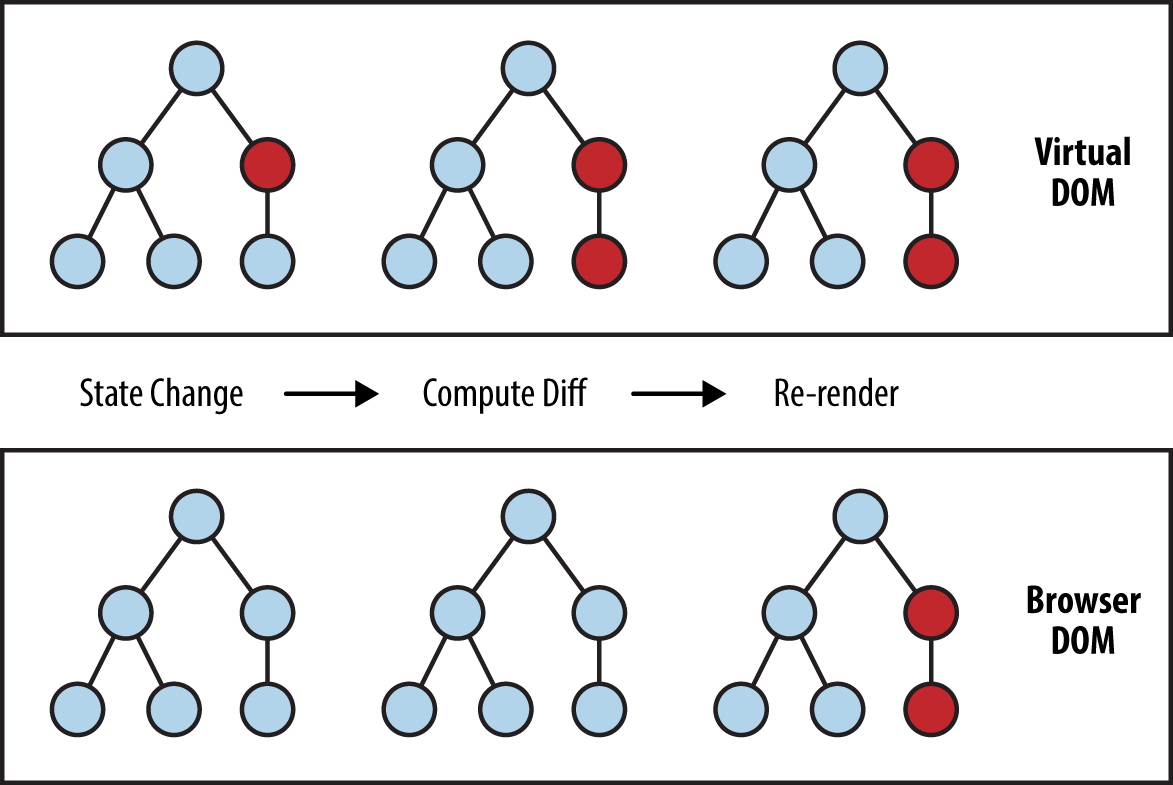
\includegraphics[width=0.8\textwidth]{images/cap4/react-virtual-dom.eps}
\caption{Funcionamiento del DOM virtual de React \cite{ReactVirtualDOM}}
\label{fig:Funcionamiento del DOM virtual de React}
\end{center}
\end{figure}

\bigskip
React es ampliamente utilizada por muchísimas empresas gracias a su capacidad de integrarse con otras librerías. 
Por ejemplo Microsoft mantuvo parte de la página en jQuery mientras iba integrando React.

\bigskip
Otro ejemplo de grandes empresas que hagan uso de esta librería son: AirBnB, Netflix, Wallmart…  \cite{ReactUsers}

\bigskip
Y muchas de ellas han contribuido al ecosistema de React, ya sea mediante guías de estilo, conjunto de componentes, patrones... \cite{ReactStyleGuide}

\bigskip
Además,la comunidad de usuarios es increíblemente activa, por ejemplo es común ver a Dan Abramov resolviendo dudas
en distintos sitios como \textit{Github} o \textit{Reddit}. Dan Abramov es el creador de Redux (una implementación de gestión de estados), desarrollador de la nueva implementación de 
React \textit{(react-fiber)}, empleado de Facebook, participante en muchas conferencias y además autor de 
múltiples herramientas como \textit{react-hot-loader}. 

\bigskip
Debido a todo lo anterior y a que además, React tiene una excelente integración con Typescript utilizando 
el formato .tsx, queda claro que es la mejor opción posible para esta aplicación. React es una librería 
desarrollada por Facebook para construir interfaces.


%++++++++++++++++++++++++++++++++++++++++++++++++++++++++++++++++++++++++++++++
\section{Tecnología para hacer la build}
\label{4:sec3}
Debido a la complejidad de las aplicaciones web modernas, es necesario 
realizar una serie de pasos intermedios entre el código original y 
el resultado final de la apliación. Para el caso de este proyecto, se debe:

\begin{itemize}

\item Compilar el código typescript a javascript.

\item Compilar el código .tsx a .jsx.

\item Resolver las importaciones de dependencias, tanto de la lógica
como de los componentes.

\item Procesar el código sass y convertirlo en css.

\end{itemize}

\subsection{Gulp/Grunt}

La primera tendencia -debido a su gran extensión- sería utilizar 
lo que se conoce como un \textit{task runner}. Actualmente, dos de los 
más conocidos son \textbf{Grunt} \cite{grunt} y  \textbf{Gulp} \cite{gulp}.

\bigskip
Ambos están basados en NodeJs y son compatibles entre sí en gran medida.
Su funcionamiento es sencillo, en un gruntfile o gulpfile se definen las tareas a
ejecutar, seleccionando los ficheros de fuente sobre los que actuar -si cabe- y la tarea 
a realizar.

\bigskip
Existen muchisimos plugins desarrollados que permiten hacer todo tipo de tareas, desde traducir
markdown hasta minimizar el contenido de los ficheros de estilos y de javascript.

\bigskip
Sin embargo, a pesar de que esta opción era altamente atractiva debido 
a su robustez, se ha optado por probar una solución aún más moderna, \textbf{webpack}.

\subsection{Webpack}

Webpack es un \textit{empaquetador de módulos} para aplicaciones de Javascript modernas.
Cuando webpack procesa la aplicación, construye un grafo de dependencias
incluyendo todos los módulos y luego lo empaqueta en orden \cite{webpack}.  

\bigskip
Webpack incorpora de serie diversas características interesantes tales como el 
poder ejecutar un servidor de desarrollo que aplica \textit{hot reloading} sobre el código 
sin requerir refrescar la página o el poder separar el código css/js de terceros para el 
entorno de producción. 

\bigskip 
El funcionamiento de webpack puede ser extremadamente resumido y simplificado en:

\begin{itemize}

\item Partiendo de un punto de entrada, una serie de reglas sobre los distintos tipos de ficheros
activan una serie de \textit{loaders} correspondientes para procesarlos. 

\item Estos loaders pueden ser concatenados entre sí para obtener el resultado deseado, por ejemplo
podemos traducir el código typescript a es6 para luego traducir este código junto a otro a es5 mediante
babel.

\item Se aplican, si fuera necesario, el uso de plugins para tareas más complejas que se quieren aplicar sobre
todos los paquetes.

\end{itemize}

\begin{figure}[!th]
\begin{center}
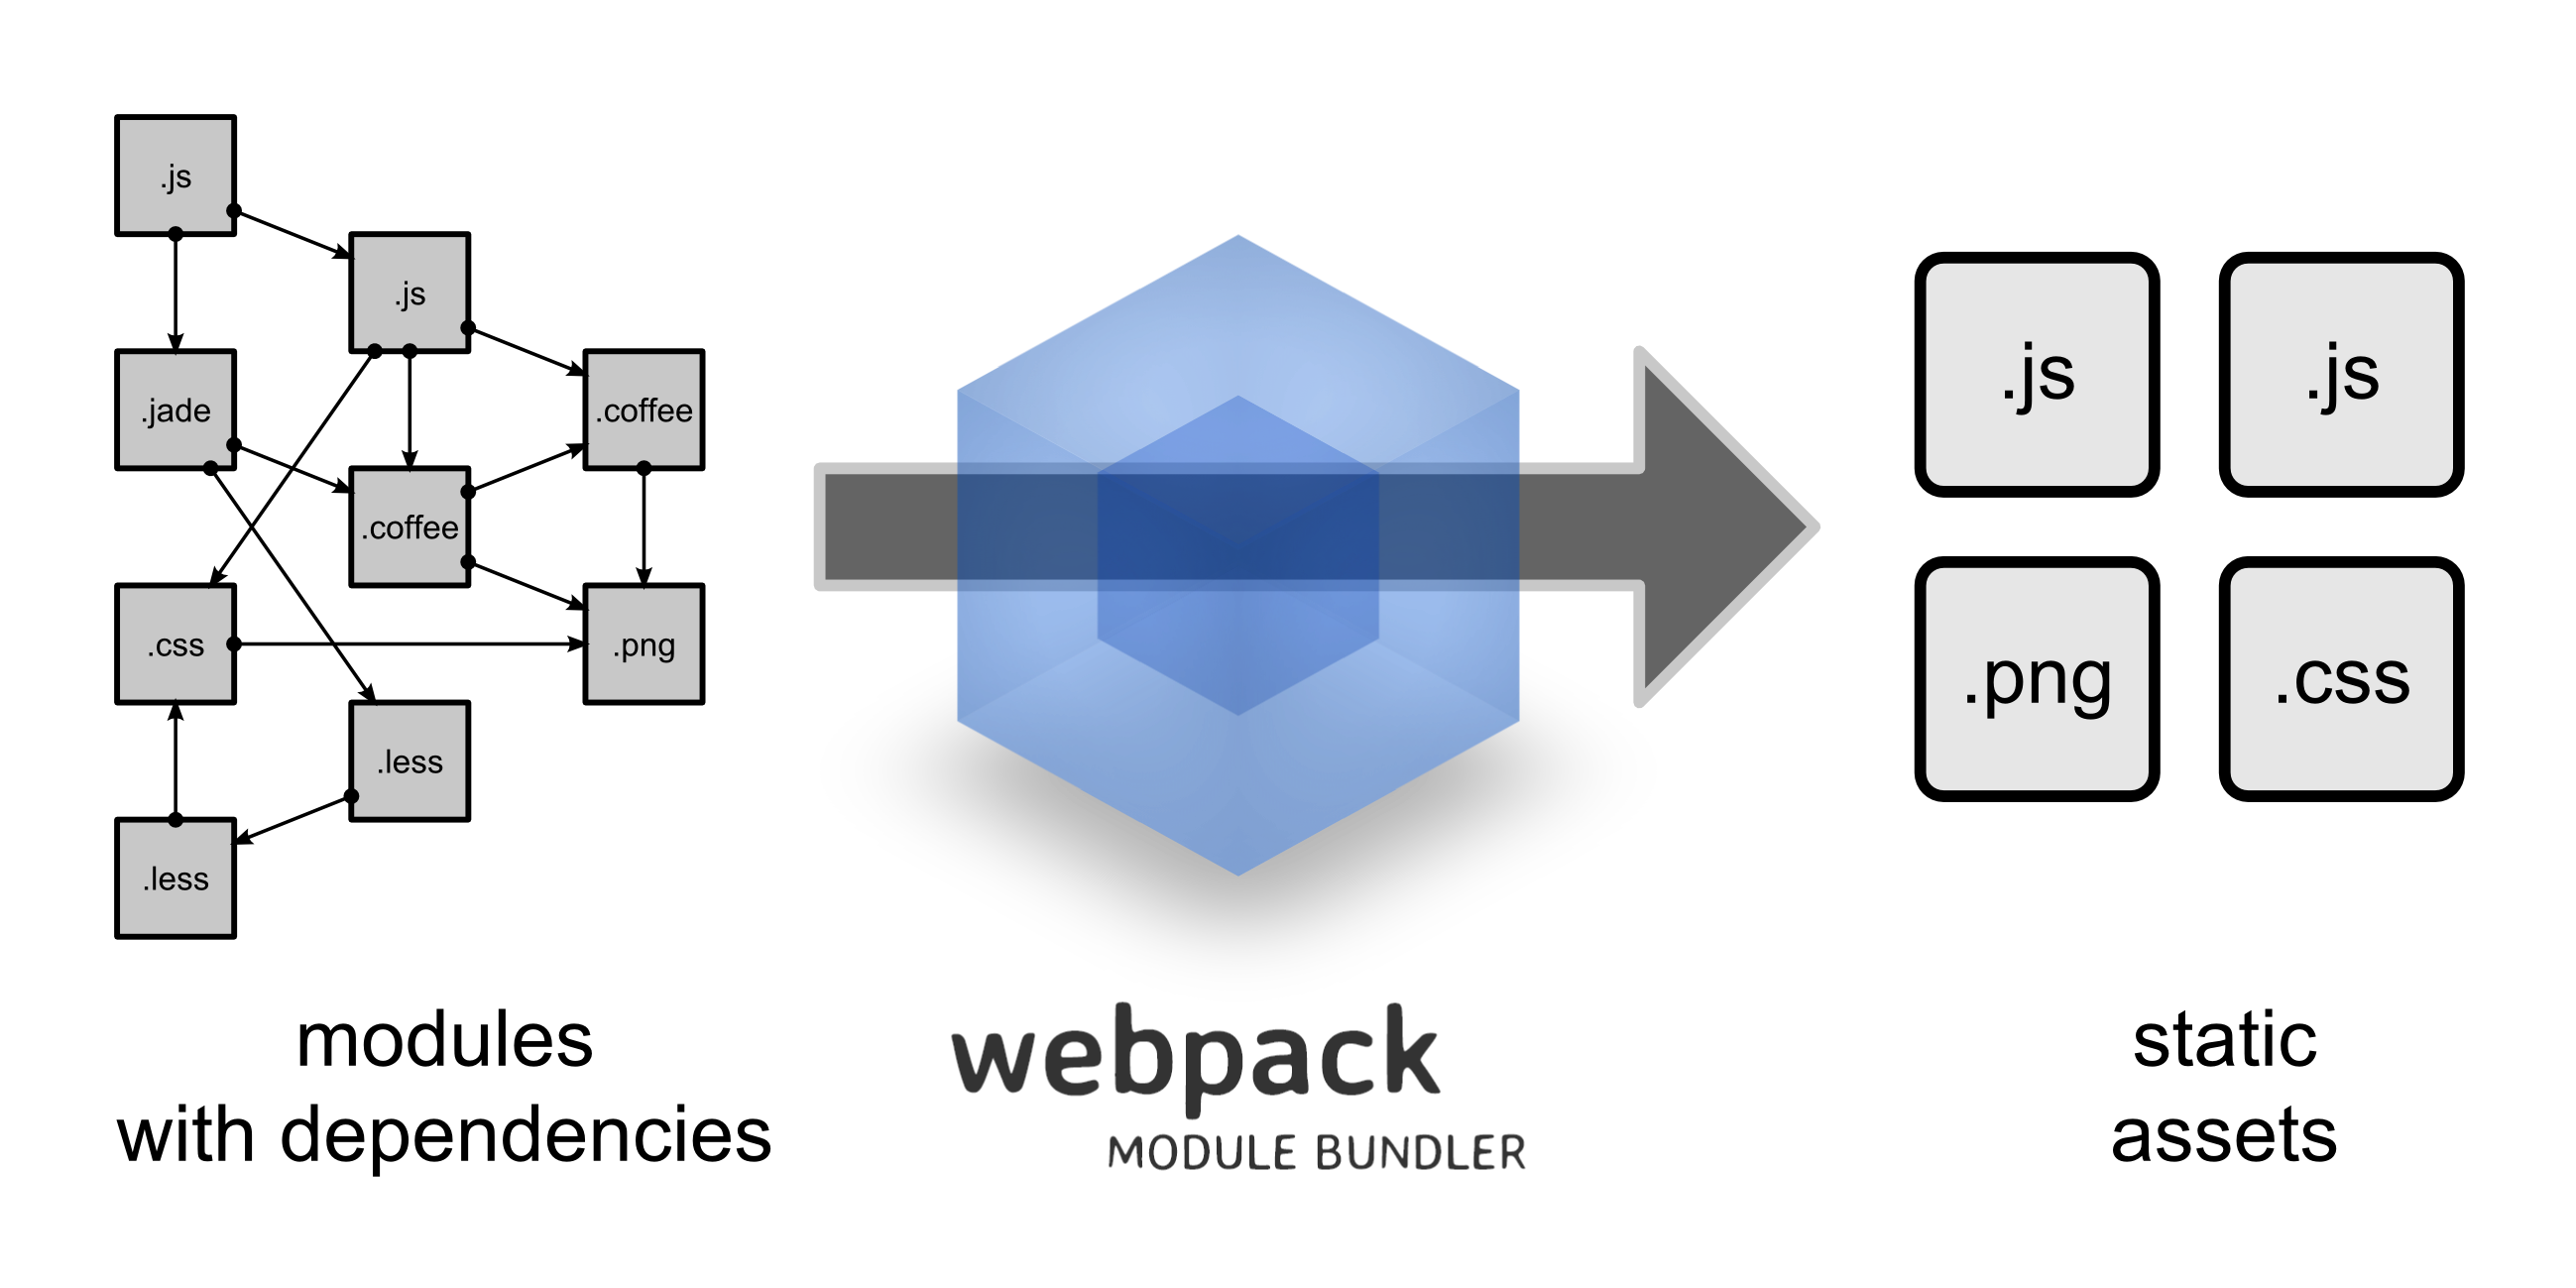
\includegraphics[width=0.8\textwidth]{images/cap4/webpack.eps}
\caption{Imagen descriptiva de Webpack}
\label{fig:Imagen descriptiva de Webpack}
\end{center}
\end{figure}


Como resultado final se obtiene una serie de paquetes que contienen todas las dependencias resueltas.

%++++++++++++++++++++++++++++++++++++++++++++++++++++++++++++++++++++++++++++++
\section{Tecnología para la documentación}
\label{4:sec4}
Para integrar la documentación en la nueva aplicación web de SIMDE resultaba obvio que esta documentación
estuviera también en formato web. Para esto existían muchas alternativas, desde un conjunto de ficheros
html hasta un pequeño sistema de gestión de contenidos. 

\bigskip
Dado que la documentación es bastante extensa pero que en realidad, no es más que un documento 
que se redactará en una ocasión y se le irán realizando pequeñas ampliaciones y/o correcciones
se optó por una solución diferente, los generadores de contenido estático.

\subsection{Generadores de contenido estático}

Los generadores de contenido estático se encargan -resumido de forma tosca y breve- de generar 
un conjunto de htmls y css a partir de una plantilla y una serie de ficheros fuentes. 

\bigskip
Este tipo de generadores estáticos tienen un gran auge entre los desarrolladores que desean 
mantener un blog -yo mismo por ejemplo, tengo uno hecho en Hugo-. 

\bigskip 
Existen múltiples ventajas de utilizar este tipo de tecnologías, pero sin duda para mi la más
importante, es que se alimentan de un formato como es el markdown. El cual es muy intuitivo de 
usar y tiene soporte más allá de este tipo de tecnologías. 

\subsection{Hexo}

Hexo es un generador de contenido estático basado en NodeJS. No posee demasiadas diferencias destacables
sobre el resto de alternativas, y ha sido escogido para este proyecto por dos motivos principales:

\begin{enumerate}

\item No me resulta desconocido, ya que lo he utilizado durante cierto tiempo.

\item Al estar basado en Javascript todo queda enfocado hacia un mismo ecosistema dando una sensación
más uniforme respecto al resto del proyecto.

\end{enumerate}


%%%%%%%%%%%%%%%%%%%%%%%%%%%%%%%%%%%%%%%%%%%%%%%%%%%%%%%%%%%%%%%%%%%%%%%%%%%%%%%
\newpage{\pagestyle{empty}}
\thispagestyle{empty}

\chapter{Desarrollo del proyecto}
\label{chapter:cinco}

%%%%%%%%%%%%%%%%%%%%%%%%%%%%%%%%%%%%%%%%%%%%%%%%%%%%%%%%%%%%%%%%%%%%%%%%%%%%%
% Chapter 5: Desarrollo del proyecto
%%%%%%%%%%%%%%%%%%%%%%%%%%%%%%%%%%%%%%%%%%%%%%%%%%%%%%%%%%%%%%%%%%%%%%%%%%%%%%%

%++++++++++++++++++++++++++++++++++++++++++++++++++++++++++++++++++++++++++++++

\section{Migración del núcleo de la aplicación}
\label{5:sec1} 

\subsection{Analizadores léxicos}
El núcleo de la aplicación se basa en el uso del generador de analizadores 
léxicos FLEX para parsear un conjunto de instrucciones similar a las del MIPS IV. 
Para realizar el proceso de migración he tenido que comprender primero el 
funcionamiento de los analizadores léxicos.

\bigskip
Un analizador léxico es un programa que recibe como entrada el código fuente de 
otro programa y produce una salida compuesta de tokens o símbolos 
que alimentarán a un analizador sintáctico.

\bigskip
Para poroceder con esta tarea se ha aislado la implementación original y se han 
realizado pequeñas pruebas concretas.

\subsection{Lex}

A pesar de las multiples librerías, que hay disponibles, se decidió que la más adecuada 
para este proyecto era Lex https://www.npmjs.com/package/lex. 

El funcionamiento de este paquete es realmente sencillo, partiendo de un 
objeto Lexer, se definen las reglas y el token a retornar. De esta forma
el código original que alimentaba flex:

// INSERTAR CODIGO original

Se ha convertido en: 

// CODIGO FLEX

%------------------------------------------------------------------------------
\section{Migración de la máquina superescalar}
\label{5:sec2} 

Una de las cosas que más puedo agradecer, es que el diseño del autor original de SIMDE era bastante 
bueno. Además, en la memoria del proyecto \textbf{CITAR MEMORIA} se incluían las decisiones de diseño
tomadas para la realización del simulador. Dando sentido.

\bigskip
Aún así, en la migración de C++ a Typescript se echaron múltiples características del primer lenguaje,
como por ejemplo: las estructuras,  la sobrecarga de operadores y el uso de iteradores sobre colecciones.

\bigskip
La mayor dificultad en esta parte del proceso era ser capaz de seguir el flujo de un volumen tan grande
de código. Por suerte, la linterna de Typescript y el \textit{intellisense} ayudaron mucho a reducir la cantidad
de pifias.

\bigskip
Aún así encontré además, algunos problemas a la hora de migrar el código debido al uso de librerías 
que no estaban en el estándar.

\textbf{CITAR FAMOSO CASO BBAS}.

\bigskip
Por comodidad durante el desarrollo, se convirtieron las estructuras de C++ en clases, de tal forma
que la gestión de las mismas fuero más sencilla.

%------------------------------------------------------------------------------
\section{Desarrollo de la interfaz}
\label{5:sec3} 

Esta tarea, aunque en un principio pudiera parecer mucho menos intensa que la migración del código 
superescalar, también ha tenido una carga de trabajo. Todo ello porque se ha intentado por encima 
de todo, conseguir un alto grado de modularización y reutilización. 

\subsection{Análisis de la interfaz original}

Si analizamos la interfaz original de SIMDE nos encontramos con esto: 

A grosso modo podríamos diferenciar 5 zonas principales.

Ahora analizaremos el funcionamiento de los componentes, en sí, con el objetivo de aislar conceptos
/funcionalidades.

\subsection{El nuevo diseño web}

A día de hoy 

\bigskip
Ahora surge un problema, ¿merece el esfuerzo aplicar el diseño de las ventanas redimensionables y 
arrastables? La conclusión es que no. SIMDE muestra la información que necesitamos. En un 
principio nos interesa ver la ejecución en sí. Luego, en su realización, nos interesa ver simplemente
el resultado de la ejecución.

\bigskip
Por eso, se ha decidido separar la ejecución de los registros / memoria mediante el uso de pestañas.

a) Pestaña 1.

b) Pestaña 2.

\subsection{El nuevo diseño por componentes}

%------------------------------------------------------------------------------
\section{Integración interfaz - lógica desarrollada}
\label{5:sec4} 

\subsection{Realización de los bindings}
Uno de los puntos a favor de haber utilizado este tipo de librerías es que su elevada flexibilidad
nos otorga cierto grado de 

%------------------------------------------------------------------------------
\section{Migración de la documentación}
\label{5:sec5} 

La primer ampliación ha sido la incorporación de documentación del programa. Aunque el
término de ampliación no es del todo correcto, puesto que en el proyecto original el autor
elaboró una extensa documentación, esta quedó inaccesible.

\bigskip
La documentación fue realizada en formato .HLP, un formato de ayuda de Windows que quedó
en desuso en Windows Vista. Y esta documentación era realmente interesante, pues no sólo
contenía datos sobre la palicación, sino que incluía consejos para el desarrollo de 
aplicaciones para las distintas máquinas y además explicaba el funcionamiento de las máquinas.

\bigskip
Para recuperar esta documentación se ha utilizado una herramientas de extracción denominada
Help Decompiler. Esta herramienta de línea de comandos procesa los ficheros de ayuda de
Windows .HLP y genera un fichero de texto enriquecido con la documentación y en una carpeta
externa el contenido multimedia que incluye la misma.

\bigskip
Para poder llevar a cabo la tarea de la documentación de forma paralela se consideró que lo mejor era
hacer un proyecto aparte. Resultaba evidente que la documentación de una aplicación web debía de estar en la
web. 

\bigskip
Tras barajar algunas opciones, se optó por mover la documentación a un formato mantenible como 
es markdown. Y partiendo de esto se utilizó un generador de contenido estático basado en NodeJS (Hexo)
para convertir este markdown en web. Se desarrollo un tema simple y personalizado para la ayuda y se 
añadió la capacidad de cambiar entre inglés y español.

\bigskip
Este es el estado actual de la aplicación de la documentación.

    IMAGEN DOCUMENTACIÓN

\bigskip
Se puede acceder a ella desde el menú \textit{Ayuda > Documentación} en la nueva aplicación del SIMDE.
%++++++++++++++++++++++++++++++++++++++++++++++++++++++++++++++++++++++++++++++


%%%%%%%%%%%%%%%%%%%%%%%%%%%%%%%%%%%%%%%%%%%%%%%%%%%%%%%%%%%%%%%%%%%%%%%%%%%%%%%
\newpage{\pagestyle{empty}}
\thispagestyle{empty}

\chapter{Ampliación de funcionalidades}
\label{chapter:seis}

%%%%%%%%%%%%%%%%%%%%%%%%%%%%%%%%%%%%%%%%%%%%%%%%%%%%%%%%%%%%%%%%%%%%%%%%%%%%%
% Chapter 6: Ampliación de funcionalidades
%%%%%%%%%%%%%%%%%%%%%%%%%%%%%%%%%%%%%%%%%%%%%%%%%%%%%%%%%%%%%%%%%%%%%%%%%%%%%%%

%++++++++++++++++++++++++++++++++++++++++++++++++++++++++++++++++++++++++++++++

En este proyecto de fin de grado se han realizado tres mejoras sobre las 
funcionalidades originales del simulador. Todas ellas han sido consecuencia
de haber utilizado la aplicación original.

%++++++++++++++++++++++++++++++++++++++++++++++++++++++++++++++++++++++++++++++
\section{Parseador}
\label{6:sec1}
Una de las características más deseadas por parte de los usuarios de SIMDE 
(entre los que yo mismo me puedo incluir), es un sistema de errores más descriptivo. 

\bigskip
Por desgracia, en la versión original de SIMDE sólo se mostraba una notificación que indicaba
que el código cargado contenía errores.

\begin{figure}[!th]
\begin{center}
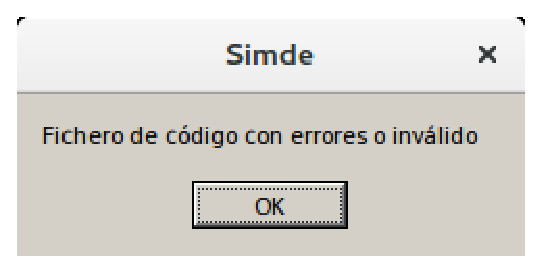
\includegraphics[width=0.5\textwidth]{images/cap6/errorsimde.eps}
\caption{Notificacion de error original SIMDE}
\end{center}
\end{figure}

Ahora, tras una serie de modificaciones en el parseador de código, se muestran los siguientes errores:

\begin{enumerate}
\item \textbf{Operando erróneo}.
\item \textbf{Opcode desconocido}.
\item \textbf{Etiqueta repetida}.
\end{enumerate}

Además, se muestra la línea del error. Esto resulta tremendamente importante, 
ya que uno de los ejercicios que se propone en SIMDE consiste en realizar mejoras en el rendimiento
de código haciendo uso de técnicas como el \textit{desenrollado de bucles}, que dan lugar a códigos de considerable
longitud.

\begin{figure}[!th]
\begin{center}
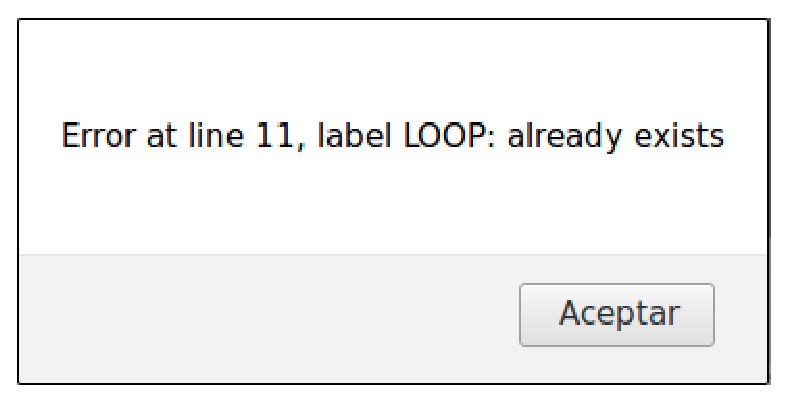
\includegraphics[width=0.5\textwidth]{images/cap6/nuevoerrorsimde.eps}
\caption{Ejemplos de errores en la nueva versión de simde}
\end{center}
\end{figure}


%++++++++++++++++++++++++++++++++++++++++++++++++++++++++++++++++++++++++++++++
\section{Modo de ejecución en lotes}
\label{6:sec2}
Otra característica deseable por parte de los usuarios es no tener el 
límite de velocidad de simulación que tiene la versión original.

\bigskip
Es común proponer ejercicios a los alumnos en los que se apliquen algoritmos de ordenación. Estos 
ejercicios tienen una cantidad media de ciclos que pueden incluso superar 500 ciclos, requiriendo
 un tiempo medio de ejecución de 2 a 3 minutos.

\bigskip
Este tiempo sumado a la necesidad de hacer medias,  a las múltiples pruebas, a la depuración de errores,
y a las distintas optimizaciones, hacen que se desperdicie una considerable cantidad de 
tiempo de forma innecesaria en tareas secundarias, distrayendo al alumno del objetivo original.

\bigskip
Es por eso que ahora, cuando el campo de velocidad está en 0 se ejecuta la simulación a velocidad 
máxima, actualizando la interfaz gráfica solamente cuando termina la ejecución. 

%++++++++++++++++++++++++++++++++++++++++++++++++++++++++++++++++++++++++++++++
\section{Histórico}
\label{6:sec3}
Otra característica que resultaba necesaria en el simulador y que se añoraba sobre todo en el primer
contacto era la posibilidad de ir hacia atrás.

\bigskip
En un principio, se esperaba utilizar algún sistema gestor de estados y permitir el time traveling. 
Por desgracia debido al volumen de este trabajo de fin de grado decidió no utilizarse este tipo de 
soluciones.

\bigskip
Sin embargo, la idea del \textit{time traveling} resultaba más que deseable, por lo que se implementó
de una forma un tanto rústica. Para permitir emular este comportamiento y mantener la fidelidad de 
la ejecución (recordemos que existen una serie de operaciones que son sujetas a un porcentaje de fallos
aleatorios), lo que se hizo fue acumular el estado visual de la máquina, el modelo en sí con el 
que se dibujaban los componentes.

\bigskip
De tal forma, cuando un usuario entraba en este modo timetraveling recorre un array de estados de la 
interfaz, imprimiendo la información almacenada, sin afectar al comportamiento de la máquina, pero 
emulando ese \textit{time traveling} de cara al usuario.

\bigskip
Por tanto, se considera que un usuario que retroceda X pasos, deberá avanzar esos X pasos para continuar
la ejecución (o en su defecto, pulsar el botón \textbf{Play}). Esto es así porque aunque como repito, se 
trata de una característica enormemente deseada en la primera toma de contacto del simulador, no se trata
de una característica de la que se espere que el usuario abuse.


%%%%%%%%%%%%%%%%%%%%%%%%%%%%%%%%%%%%%%%%%%%%%%%%%%%%%%%%%%%%%%%%%%%%%%%%%%%%%%%
\newpage{\pagestyle{empty}}
\thispagestyle{empty}

\chapter{Conclusiones y líneas futuras }
\label{chapter:Conclusiones}

%%%%%%%%%%%%%%%%%%%%%%%%%%%%%%%%%%%%%%%%%%%%%%%%%%%%%%%%%%%%%%%%%%%%%%%%%%%%%
% Chapter 7: Conclusiones y Trabajos Futuros 
%%%%%%%%%%%%%%%%%%%%%%%%%%%%%%%%%%%%%%%%%%%%%%%%%%%%%%%%%%%%%%%%%%%%%%%%%%%%%%%
\section{Conclusiones}
\label{7:sec1}

Con el desarrollo de este trabajo se ha conseguido disponer de una nueva versión
del simulador de paralelismo a nivel de instrucción SIMDE \cite{NuevaURLSimde}. 

Se ha visto además que las múltiples herramientas y tecnologías disponibles hoy
día (los nuevos lenguajes transpilables a javascript, los web components, las 
herramientas para la distribución), permiten elaborar y diseñar con relativa
facilidad aplicaciones que se salen de la norma.

Es necesario recordar que, como en todo proceso de software, el desarrollo de una 
aplicación está vivo, sujeto a cambios y dado el impresionante ritmo al que evoluciona
el mundo web, es posible que en un futuro aparezcan alternativas que permitan mejorar 
la experiencia de este simulador.

%++++++++++++++++++++++++++++++++++++++++++++++++++++++++++++++++++++++++++++++
\section{Líneas futuras}
\label{7:sec2}

Tras el desarrollo de este trabajo se abren varias líneas futuras: 

\begin{itemize}

\item Implementación de la máquina VLIW: Con el desarrollo de este trabajo de fin de grado también se han implementado las estructuras básicas que se comparte con la máquina 
VLIW. Esta línea de trabajo tiene la mayor prioridad, pues equipara la funcionalidad de la aplicación web de 
SIMDE a la aplicación original.

\item Realizar una mayor cantidad de test: En el mundo web no resulta sencillo realizar test 
para los distintos casos, sin embargo, la lógica que acompaña al simulador es un gran candidato a 
ser testeado. Con las bases asentadas en los tests realizados para la estructura de la cola y 
del parseador del código, se podría extender este funcionamiento a pequeñas simulaciones.

\item Implementar un sistema de gestión de estados: En la aplicación actual se ha hecho un sistema
de estados simple debido al volumen de trabajo que requiere incorporar tecnologías
como Redux y a las dificultades que entrañan los Observables que vienen 
en un sistema como Mobx. En líneas futuras este sistema podría sustituirse por un 
sistema más robusto desarrollado por terceros.

\item Intregar tutoriales de funcionamiento: Ahora que SIMDE es una aplicación con un gran
grado de accesibilidad, la única barrera a la que se enfrentan sus usuarios es a la dificultad de
comprender lo que están visualizando y el objetivo en sí de la máquina. A pesar de que esto
se explica en la documentación la integración de pequeños tutoriales de funcionamiento acabaría con 
esta barrera inicial y fomentaría el uso a gente con un menor conocimiento específico del campo
de arquitectura de computadores.

\item Automatizar el sistema de ejercicios: También con el objetivo de fomentar la autonomía podría
resultar interesante automatizar el sistema de ejercicios, de esta forma, mediante el uso de alguna
tecnología en \textit{backend} se podría no solo entregar al alumno un problema a resolver sino 
comparar la solución que ha propuesto con algunas soluciones propuestas por los profesores de antemano
de tal forma que el alumno sea capaz de recibir una retroalimentación instántanea sobre su solución.

\item Incluir gamificación: Mediante la incorporación de dinámicas de juego, se podría fomentar la
competitividad entre los usuarios, premiando la creatividad para la resolución de problemas e instando
a los alumnos a comprender mejor las arquitecturas de las máquinas y sus ventajas y limitaciones para
obtener códigos que requieran menor tiempo de ejecución.

\item Permitir el desarrollo colaborativo: Dado que uno de los requisitos principales de un 
ingeniero informático es la capacidad de trabajar en equipo, una línea de desarrollo interesante
en este sentido sería sincronizar la ejecución de las máquinas entre varios miembros de un grupo
mediante el uso de websockets. Así pues, si además se incluyera alguna herramienta de comunicación
 como un chat, se lograría fomentar una buena practica entre los alumnos y se dotaría de cierto
 dinamismo al desarrollo.

\item Desarrollar más simuladores: Con el desarrollo de este simulador se asientan las bases para
el futuro desarrollo de múltiples simuladores que permitan enseñar de forma interactiva
diversos fundamentos de la arquitectura de computadores como por ejemplo la el paralelismo a nivel 
de hilo o la coherencia a nivel de cache en sistemas multiproceso.

\end{itemize}

%%%%%%%%%%%%%%%%%%%%%%%%%%%%%%%%%%%%%%%%%%%%%%%%%%%%%%%%%%%%%%%%%%%%%%%%%%%%%%%
\newpage{\pagestyle{empty}}
\thispagestyle{empty}

\chapter{Summary and Conclusions }
\label{chapter:ingles}

%%%%%%%%%%%%%%%%%%%%%%%%%%%%%%%%%%%%%%%%%%%%%%%%%%%%%%%%%%%%%%%%%%%%%%%%%%%%%
% Chapter 8: Summary and Conlusions
%%%%%%%%%%%%%%%%%%%%%%%%%%%%%%%%%%%%%%%%%%%%%%%%%%%%%%%%%%%%%%%%%%%%%%%%%%%%%%%

%---------------------------------------------------------------------------------
\section{Summary}
\label{8:sec:1}

With the development of this work we have now available a new versión of
the Instruction Level Paralelism simulator SIMDE.

\bigskip
It has also been seen that the many tools and technologies available today (the new languages 
for the web, the webcomponents and the building tools), allowing to develop 
and design with relative ease complex applications.

\bigskip
It is necessary to remember that, as in all software processes, the development of a
application is alive, subject to changes and given the impressive pace at which the web world evolves.
It is possible that in the future there will be alternatives to improve the experience of this simulator.

%---------------------------------------------------------------------------------
\section{Future work lines}
\label{8:sec:2}

After the development of this work, several futurel lines are opened: 

\begin{itemize}

\item Implementation of the Very Long Instruction Word machine: Based on the initial design,
the application is ready for evolve and get the same capabilities that original simulator.
This line has the greatest priority since it equates the functionality of SIMDE's web application to
the original application.

\item Make a greater amount of test: In the web world is not easy to test 
 the multiple cases, however this application is a great candidate to be tested. 
As the basis for this laid in the tests made for the Code and the Queue structure,
the test could be extended to small simulations.

\item Implement a state management system: In the current application a simple management state system
have been used due to the high amount of work required to incorporate technologies such as Redux and 
the difficulties involved in the use of Observables in a system like Mobx. In future lines this system could be
replaced by a more robust system developed by third parties.

\item Include operating tutorials: Now that SIMDE is an application with great accessibility,
the only barrier faced by its users is the difficulty of understandoing what they are 
visualizing and the objective of the simulator itself. Although this is explained in the 
documentation the integration of small tutorials would put an end to this initial barrier
and would encourage the use to people with a less specific knowledge of the field
of computer architecture.

\item Automate the exercise system: With the aim of promoting autonomy could be interesting 
to automate the exercise system. By using some technology in the \textit{backend}, the student
could be given not only a problem to solve but the possibility of compare the solution 
he has proposed with some solutions made by the teachers beforehand. With that the student
could receive an important feedback instantly.

\item Include gamification: By incorporating gaming dynamics,competitiveness among users would promoted. 
Rewarding creativity for problem solving and urging students to understand the architectures 
of the machines and their advantages and limitations in order orden to develop codes 
that require less execution time.

\item Allow collaborative development: Since one of the main requirements of a
computer engineer is the ability to work in a team, an interesting development line
in this sense would be to synchronize the execution of the machines between several members of a group
through the use of websockets. Thus, if also some communication tool as a chat is included,
it would be possible to promote good practises among the students and it would provide 
dynamism to development.

\item Develop more simulators: With the development of this simulator, the basis are laid for
the future development of multiple simulators that allow to teach interactively multiple computer architecture's foundations
such as level thread parallelism or cache coherence in multiprocess systems.

\end{itemize}

%%%%%%%%%%%%%%%%%%%%%%%%%%%%%%%%%%%%%%%%%%%%%%%%%%%%%%%%%%%%%%%%%%%%%%%%%%%%%%%
\newpage{\pagestyle{empty}}
\thispagestyle{empty}

\chapter{Presupuesto}
\label{chapter:Presupuesto}

%%%%%%%%%%%%%%%%%%%%%%%%%%%%%%%%%%%%%%%%%%%%%%%%%%%%%%%%%%%%%%%%%%%%%%%%%%%%%
% Chapter 9: Presupuesto
%%%%%%%%%%%%%%%%%%%%%%%%%%%%%%%%%%%%%%%%%%%%%%%%%%%%%%%%%%%%%%%%%%%%%%%%%%%%%%%

%--------------------------------------------------------------------------
\begin{table}[!ht]
\begin{center}
\begin{tabular}{|p{80mm}|p{40mm}|} \hline 
\textbf{Descripción } & \textbf{Coste} \\ \hline
200 Horas de trabajo &
8000 \euro
\\
\hline

Ordenador para desarrollo &
1300 \euro
\\
\hline

Total &
9300 \euro
\\
\hline

\end{tabular}
\end{center}
\caption{Presupuesto}
\label{table:resOthers}
\end{table}




%%%%%%%%%%%%%%%%%%%%%%%%%%%%%%%%%%%%%%%%%%%%%%%%%%%%%%%%%%%%%%%%%%%%%%%%%%%%%%%

%%%%%%%%%%%%%%%%%%%%%%%%%%%%%%%%%%%%%%%%%%%%%%%%%%%%%%%%%%%%%%%%%%%%%%%%%%%%%%%
\newpage{\pagestyle{empty}}
\thispagestyle{empty}
\begin{appendix}

\chapter{Título del Apéndice 1}
\label{appendix:1}
\section{Algoritmo XXX}
\label{Apendice1:XXX}

\begin{center}
\begin{footnotesize}
\begin{verbatim}

***********************************************************************************
*
* Fichero .h
*
***********************************************************************************
*
* AUTORES
*   
*
* FECHA
*   
*
* DESCRIPCION
*   
*
************************************************************************************/

\end{verbatim}
\end{footnotesize}
\end{center}

\section{Algoritmo YYY}
\label{Apendice1:YYY}

\begin{center}
\begin{footnotesize}
\begin{verbatim}


/***********************************************************************************
 *
 * Fichero .h
 *
 ***********************************************************************************
 *
 * AUTORES
 *
 * FECHA
 *
 * DESCRIPCION
 *
 *
 ************************************************************************************/

\end{verbatim}
\end{footnotesize}
\end{center}


\end{appendix}

%%%%%%%%%%%%%%%%%%%%%%%%%%%%%%%%%%%%%%%%%%%%%%%%%%%%%%%%%%%%%%%%%%%%%%%%%%%%%%%
\addcontentsline{toc}{chapter}{Bibliografía}
\bibliographystyle{plain}

\bibliography{memtfg}
\nocite{*}

%%%%%%%%%%%%%%%%%%%%%%%%%%%%%%%%%%%%%%%%%%%%%%%%%%%%%%%%%%%%%%%%%%%%%%%%%%%%%%%

\end{document}
